\documentclass[a4paper, 11pt]{article}

\usepackage{amsmath}
\usepackage{graphicx}
\usepackage[portuges]{babel}
\usepackage[utf8x]{inputenc}
\usepackage{comment}
\usepackage{fullpage}

\usepackage{listings}
\usepackage{color}
\definecolor{mygreen}{RGB}{28,172,0}
\definecolor{mylilas}{RGB}{170,55,241}


\begin{document}

\noindent
\large\textbf{Lista de Exercícios 4} \hfill \textbf{Luis Vinicius Costa Silva} \\
\normalsize Modelagem Computacional \\
Prof. Thiago Alves de Queiroz \\
\hfill Data de Entrega: 07/09/2018

\subsection*{Questão 1}
Um algoritmo que resolve um sistema linear utilizando o método de Eliminação de Gauss com substituição inversa foi escrito, as chamadas abaixo do programa ``ex1.m" resolvem a Letra A e B da 
Questão 1 (o primeiro argumento é a matriz de coeficientes enquanto que o segundo argumento é o vetor de termos independentes):

\begin{lstlisting}[language=bash]
./ex1.m "[2 ,0, 0, 0;1 ,1.5,0,0;0,-3, 0.5,0;2,-2,1,1]" "[3,4.5,-6.6,0.8]"
\end{lstlisting}

\begin{lstlisting}[language=bash]
./ex1.m "[1,1,0,1;2,1,-1,1;4,-1,-2,2;3,-1,-1,2]" "[2,1,0,-3]"
\end{lstlisting}

A primeira chamada do programa computou a seguinte solução para o sistema de equações:

$$
\left\{\begin{matrix}
x_1 = 1.5\\ 
x_2 = 2.0\\ 
x_3 = -1.2\\ 
x_4 = 3.0 \\ 
\end{matrix}\right.
$$

Enquanto que a segunda chamada do programa retorna a seguinte solução:

$$
\left\{\begin{matrix}
x_1 = NaN\\ 
x_2 = NaN\\ 
x_3 = \infty\\ 
x_4 = -\infty \\ 
\end{matrix}\right.
$$
O array retornado ante a segunda chamada do programa demonstra que o sistema de equações da letra B é impossível. Não houve necessidade de permutar linhas durante a execução das duas chamadas a fim de que o sistema fosse resolvido.

\subsection*{Questão 2}
A questão 2 foi resolvido através do algoritmo abaixo:

\lstset{language=Matlab,%
    %basicstyle=\color{red},
    breaklines=true,%
    morekeywords={matlab2tikz},
    keywordstyle=\color{blue},%
    morekeywords=[2]{1}, keywordstyle=[2]{\color{black}},
    identifierstyle=\color{black},%
    stringstyle=\color{mylilas},
    commentstyle=\color{mygreen},%
    showstringspaces=false,%without this there will be a symbol in the places where there is a space
    numbers=left,%
    numberstyle={\tiny \color{black}},% size of the numbers
    numbersep=9pt, % this defines how far the numbers are from the text
    emph=[1]{for,end,break},emphstyle=[1]\color{red}, %some words to emphasise
}

\begin{lstlisting}
b = [-2,3,2]; 
for k=-10:0.1:10
 L = k;
 A = [1,-1, L; -1, 2, -L; L, 1, 1];
 
 %printf("Para L=%f, temos:\n",L);
 %disp([A,b']);
 _flag = AvaliaFactibilidadeDoSistema(A,b);
 if _flag==0
  printf("\nPara L=%f, temos: SPD\n\n",k);
 elseif _flag==1
  printf("\nPara L=%f, temos: SPI\n\n",k);
 else
  printf("\nPara L=%f, temos: SI\n\n",k);
 endif
endfor
\end{lstlisting}

E as seguintes chamadas:

\begin{lstlisting}[language=bash]
./ex2.m | grep SPD
\end{lstlisting}

\begin{lstlisting}[language=bash]
./ex2.m | grep SPI
\end{lstlisting}

\begin{lstlisting}[language=bash]
./ex2.m | grep SI
\end{lstlisting}

Para $\alpha=-1$, temos que o sistema é possível determinado, enquanto que para $\alpha=1.0$ temos que o sistema é impossível, para qualquer outro $\alpha$, temos que o 
sistema é possível determinado.\newline
Basicamente este algoritmo percorre um intervalo considerável a um passo $h$, e checa se a matriz é positiva definida a cada passo da iteração, o comando ``grep" simplesmente facilita a
percepção de quais intervalos correspondem a cada tipo de sistema de equações (i.e: Sistema impossível (SI), Sistema Possível Determinado (SPD), Sistema Impossível Indeterminado (SPI)).

\subsection*{Questão 4}
Utilizando a regra de Laplace, o determinante é computado através das submatrizes:
\subsubsection*{Letra A}
$$
A = \begin{vmatrix}
1 & 2  & 0 \\ 
2 & 1 & -1 \\ 
3 & 1 & 1 \\
\end{vmatrix}
$$
\begin{center}
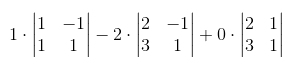
\includegraphics[width=0.5\textwidth]{q4a1.png}
\end{center}

\begin{center}
$det(A) = 1\cdot \:2-2\cdot \:5+0\cdot \left(-1\right)=-8$
\end{center}


\subsubsection*{Letra B}
Já que a regra de Laplace é demasiada trabalhosa para matrizes de dimensão maior que 3, o determinante foi calculado através do escalonamento da matriz inicial e o posterior produtório dos elementos
da diagonal principal:
$$
A = \begin{vmatrix}
2 & 0 & 1 & 2 \\ 
1 & 1 & 0 & 2 \\ 
2 & -1 & 3 & 1 \\
3 & -1 & 4 & 3 \\
\end{vmatrix}
$$


$$
\phantom{A = }
\begin{vmatrix}
3 & -1 & 4 & 3 \\ 
1 & 1 & 0 & 2 \\ 
2 & -1 & 3 & 1 \\
2 & 0 & 1 & 2 \\ 
\end{vmatrix}
R_1 \leftrightarrow R_4
$$

$$
\phantom{A = }
\begin{vmatrix}
3 & -1 & 4 & 3 \\ 
0 & \frac{4}{3} & -\frac{4}{3} & 1 \\ 
2 & -1 & 3 & 1 \\
2 & 0 & 1 & 2 \\ 
\end{vmatrix}
R_2 \leftarrow R_2-\frac{1}{3} \cdot R_1
$$

$$
\phantom{A = }
\begin{vmatrix}
3 & -1 & 4 & 3 \\ 
0 & \frac{4}{3} & -\frac{4}{3} & 1 \\ 
0 & -\frac{1}{3} & \frac{1}{3} & -1 \\
2 & 0 & 1 & 2 \\ 
\end{vmatrix}
R_3 \leftarrow R_3-\frac{2}{3} \cdot R_1
$$

$$
\begin{vmatrix}
3 & -1 & 4 & 3 \\ 
0 & \frac{4}{3} & -\frac{4}{3} & 1 \\ 
0 & -\frac{1}{3} & \frac{1}{3} & -1 \\
0 & \frac{2}{3} & -\frac{5}{3} & 0 \\ 
\end{vmatrix}
R_4 \leftarrow R_4-\frac{2}{3} \cdot R_1
$$

$$
\begin{vmatrix}
3 & -1 & 4 & 3 \\ 
0 & \frac{4}{3} & -\frac{4}{3} & 1 \\ 
0 & 0 & 0 & -\frac{3}{4} \\
0 & \frac{2}{3} & -\frac{5}{3} & 0 \\ 
\end{vmatrix}
R_3 \leftarrow R_3+\frac{1}{4} \cdot R_2
$$

$$
\begin{vmatrix}
3 & -1 & 4 & 3 \\ 
0 & \frac{4}{3} & -\frac{4}{3} & 1 \\ 
0 & 0 & 0 & -\frac{3}{4} \\
0 & 0 & -1 & -\frac{1}{2} \\ 
\end{vmatrix}
R_4 \leftarrow R_4-\frac{1}{2} \cdot R_2
$$

$$
\begin{vmatrix}
3 & -1 & 4 & 3 \\ 
0 & \frac{4}{3} & -\frac{4}{3} & 1 \\ 
0 & 0 & -1 & -\frac{1}{2} \\
0 & 0 & 0 & -\frac{3}{4} \\ 
\end{vmatrix}
R_3 \leftrightarrow R_4
$$

$$det(A) = \cdot \frac{4}{3} \cdot (-1) \cdot -\frac{3}{4} = 3$$
$$det(A) = 3$$

\subsection*{Questão 5}
De forma similar a Questão 2, o algoritmo abaixo foi escrito a fim de aferir para qual $\alpha$, a matriz seria singular:
\lstset{language=Matlab,%
    %basicstyle=\color{red},
    breaklines=true,%
    morekeywords={matlab2tikz},
    keywordstyle=\color{blue},%
    morekeywords=[2]{1}, keywordstyle=[2]{\color{black}},
    identifierstyle=\color{black},%
    stringstyle=\color{mylilas},
    commentstyle=\color{mygreen},%
    showstringspaces=false,%without this there will be a symbol in the places where there is a space
    numbers=left,%
    numberstyle={\tiny \color{black}},% size of the numbers
    numbersep=9pt, % this defines how far the numbers are from the text
    emph=[1]{for,end,break},emphstyle=[1]\color{red}, %some words to emphasise
}

\begin{lstlisting}
L = 0;
h = 0.01;
A = [1,2,-1;1,L,1;2,L,-1];
for i=-10:h:10
L = i;
A = [1,2,-1;1,L,1;2,L,-1];
if isinf(inv(A))
 printf("\nPara L=%f, temos que a matriz abaixo eh singular:\n",L);
 disp(A);
endif
endfor
\end{lstlisting}
Basicamente, o algoritmo varia o $\alpha$ da matriz $A$ através de um passo $h$, e a cada iteração, checa se a matriz gerada não possui inversa, caso esta condição seja satisfeita,
um valor de $\alpha$ que torna a matriz singular é descoberto e impresso. Neste caso, a matriz $A$ é singular apenas para $\alpha=6$.

\subsection*{Questão 6}
Um algoritmo para fatoração LU foi escrito, no qual a matriz A foi fatorada na forma LU, i.e: $A=LU$, abaixo as matrizes fatores de A podem ser observadas:

$$
L = \begin{bmatrix}
   1 && 0 && 0 && 0 \\
  -0.66790 &&  1.00000 && 0.00000  && 0.00000 \\
   0.36119 &&  0.14002 &&  1.00000 &&  0.00000 \\
  -0.16602 && -0.37925 && -0.51127 &&  1.00000 \\
\end{bmatrix}
$$


$$
U = \begin{bmatrix}
    6.02350  &&  7.00000   &&    0.00000   &&   -4.15610 \\
    0.00000   &&   10.67531  &&     0.00000   &&   -1.57856 \\
    0.00000  &&     0.00000   &&   -2.17320   &&    6.91886 \\
    0.00000   &&    0.00000   &&    0.00000   &&    2.24878 \\
\end{bmatrix}
$$

\subsection*{Questão 8}
O algoritmo de fatoração LDL computou a seguinte matriz triangular inferior:
$$
L = \begin{bmatrix}
   2.00000 &&  0.00000 &&  0.00000 &&  0.00000 \\
   0.50000 &&  1.65831 &&  0.00000 &&  0.00000 \\
  -0.50000 && -0.45227 &&  2.13201 &&  0.00000 \\
   0.00000 &&  0.00000 &&  0.93808 &&  1.76635 \\
\end{bmatrix}
$$

\subsection*{Questão 10}
O exercício 10 pede todos os valores possíveis de $\alpha$ de tal forma que A seja positiva definida.
$$
A = 
\begin{bmatrix}
2 & \alpha  & -1 \\ 
\alpha & 2 & 1 \\ 
-1 & 1 & 4
\end{bmatrix}
$$

Neste caso, deve-se lembrar que uma matriz é positiva definida, se somente se, seus autovalores são positivos, logo obtém-se o polinômio característico da matriz em função de $\alpha$, 
são estes $\lambda_1, \lambda_2, \lambda_3$, de tal forma que $\lambda_i>0\phantom{0}\forall \phantom{0}1\leq i \leq$ 3.


$$
P_A(x) = det(A-xI) \text{\phantom{0} onde\phantom{0}I é a matriz identidade}
$$

Após esse procedimento, é obtido:

$$
\left\{\begin{matrix}
\lambda_1 \Rightarrow 0.5\sqrt{\alpha^2+4\alpha+12} - 0.5\alpha+3 = 0\\ 
\lambda_2 \Rightarrow 3-0.5\sqrt{\alpha^2+4\alpha+12} - 0.5\alpha = 0\\ 
\lambda_3 \Rightarrow \alpha+2 = 0\phantom{\sqrt{\alpha^2+4\alpha+12} - 0.55\alpha}\\
\end{matrix}\right.
$$

Logo, o intervalo de valores de $\alpha$ que tornam $A$ positiva definida são limitados por, respectivamente, as duas raízes mínimas de $\lambda_i$. Visto que a equação $3$ é trivial, utiliza-se o método da bisseção para
obter as raízes das equações $1$ e $2$. Após obtidas as raízes das equações $1$ e $2$ podemos concluir que a matriz $A$ é positiva definida para qualquer $\alpha$ entre $-2$(Eq. $3$) e $1.5$ (Eq. $2$), i.e: $-2<\alpha<1.5$
\end{document}
